\documentclass[12pt,a4paper]{article}

 % --- Pacchetti fondamentali ---
\usepackage[utf8]{inputenc}
\usepackage[T1]{fontenc}
\usepackage[italian]{babel}
\usepackage{geometry}
\geometry{a4paper, top=2.5cm, bottom=2.5cm, left=2.5cm, right=2.5cm}
\usepackage{graphicx}
\usepackage[numbers, square]{natbib}
\usepackage[hidelinks]{hyperref}
\usepackage{cleveref} % deve venire dopo hyperref
\usepackage{float}
\usepackage{xcolor}
\usepackage{parskip}
\usepackage[font=small,labelfont=bf]{caption}
\usepackage{subcaption}
\usepackage{microtype} 
\usepackage{lmodern}
\usepackage{tabularx}

\usepackage{booktabs}

% --- Listings (Configurazione JSON) ---
\usepackage{listings}
\definecolor{codegreen}{rgb}{0,0.6,0}
\definecolor{codegray}{rgb}{0.5,0.5,0.5}
\definecolor{codepurple}{rgb}{0.58,0,0.82}
\definecolor{backcolour}{rgb}{0.95,0.95,0.92}
\definecolor{punct}{RGB}{100,100,100}
\definecolor{numb}{RGB}{0,102,204}
\definecolor{delim}{RGB}{20,105,176}
\definecolor{json_key}{RGB}{18, 110, 213}    % Blu per le chiavi
\definecolor{json_string}{RGB}{0, 153, 51}  % Verde per i valori stringa
\definecolor{json_number}{RGB}{255, 102, 0} % Arancione per i numeri

\lstdefinelanguage{json}{
    basicstyle=\ttfamily\footnotesize,
    numbers=left,
    numberstyle=\tiny\color{codegray},
    stepnumber=1,
    numbersep=8pt,
    showstringspaces=false,
    breaklines=true,
    frame=lines,
    stringstyle=\color{json_string},
    morestring=[b]",
    backgroundcolor=\color{backcolour},
    moredelim=[is][\color{json_key}]{||}{||},
    literate=
     *{0}{{{\color{json_number}0}}}{1}
      {1}{{{\color{json_number}1}}}{1}
      {2}{{{\color{json_number}2}}}{1}
      {3}{{{\color{json_number}3}}}{1}
      {4}{{{\color{json_number}4}}}{1}
      {5}{{{\color{json_number}5}}}{1}
      {6}{{{\color{json_number}6}}}{1}
      {7}{{{\color{json_number}7}}}{1}
      {8}{{{\color{json_number}8}}}{1}
      {9}{{{\color{json_number}9}}}{1}
      {:}{{{\color{punct}{:}}}}{1}
      {,}{{{\color{punct}{,}}}}{1}
      {\{}{{{\color{delim}{\{}}}}{1}
      {\}}{{{\color{delim}{\}}}}}{1}
      {[}{{{\color{delim}{[}}}}{1}
      {]}{{{\color{delim}{]}}}}{1}
}


\hypersetup{
    pdftitle={BuySellChain - Documento di Progettazione e Analisi di Sicurezza},
    pdfauthor={Salvucci Franco, Ionut Georgian Zbirciog},
    pdfsubject={Sistema d'Asta Trustless su Hyperledger Fabric},
    pdfkeywords={Blockchain, Hyperledger Fabric, Asta, Smart Contract}
}

% Ambiente "Definizione" migliorato
\newenvironment{definizione}[1][]{
    \vspace{10pt}\par\noindent\textbf{Definizione%
    \if\relax\detokenize{#1}\relax\else\ (\textit{#1})\fi.}\itshape\ }{\vspace{10pt}\par}

% --- Dati del documento ---
\title{
    \vspace{2cm}
    {\Huge\bfseries BuySellChain}\\
    \vspace{0.5cm}
    {\Large Sistema d'Asta Trustless su Blockchain Hyperledger Fabric}\\
    \vspace{1cm}
    {\small Thread Model BuySellChain }
}

\author{
    \textbf{Salvucci Franco} (Mat. 0368692) \\
    \textbf{Ionut Georgian Zbirciog} (Mat. 0381279)
}

\begin{document}

\maketitle

\tableofcontents

\newpage

\section{Definizione dell'infrastruttura e delle Zone di Sicurezza}
L'architettura di rete del sistema \textbf{BuySellChain} è stata progettata e segmentata seguendo i principi fondamentali dello standard internazionale IEC 62443. Questa suddivisione in zone logiche di sicurezza (Security Zones) e condotti di comunicazione (Conduits) permette di isolare i sistemi critici, limitare drasticamente i movimenti laterali di un eventuale attaccante in caso di compromissione perimetrale e applicare policy di accesso granulari basate sul principio del minimo privilegio (Least Privilege).

\subsection{Zona DMZ (Demilitarized Zone)}
La DMZ funge da livello cuscinetto tra la rete pubblica (Internet) e la rete interna strettamente confinata. Il suo scopo è ricevere, filtrare e sanitizzare tutte le richieste provenienti dall'esterno prima che queste possano raggiungere i sistemi di validazione e persistenza dei dati.

\begin{table}[h]
\centering
\small
\renewcommand{\arraystretch}{1.4}
\begin{tabularx}{\textwidth}{>{\hsize=0.3\hsize\bfseries}X >{\hsize=0.7\hsize}X}
\toprule
Componente & Descrizione e Funzione Architetturale \\
\midrule
Reverse Proxy (es. NGINX) & Gestisce la terminazione TLS/SSL, isolando i server applicativi dall'esposizione diretta. Fornisce funzionalità di bilanciamento del carico e mitigazione base contro attacchi volumetrici (DDoS). \\
Security Gateway (Backend) & Server applicativo sviluppato in Python/Flask. Agisce come Policy Enforcement Point (PEP): valida i token JWT, implementa il controllo degli accessi (RBAC) e sanitizza gli input strutturali (JSON Schema) prima di invocare i comandi verso la blockchain. \\
Gestore delle Sessioni & Modulo integrato nel Gateway per l'emissione, la validazione e la revoca dei JSON Web Token (JWT), gestendo le transizioni di stato dell'autenticazione in modalità stateless. \\
\bottomrule
\end{tabularx}
\caption{Componenti dell'infrastruttura situati nella Zona DMZ.}
\end{table}

\newpage

\subsection{Zona IT / Enterprise (Restricted Zone)}
Questa zona, non accessibile direttamente dall'esterno, ospita i motori di persistenza, il sistema di consenso decentralizzato e i dati sensibili. Le comunicazioni in ingresso sono consentite esclusivamente dal Security Gateway tramite protocolli e porte rigorosamente definiti.

\begin{table}[h]
\centering
\small
\renewcommand{\arraystretch}{1.4}
\begin{tabularx}{\textwidth}{>{\hsize=0.3\hsize\bfseries}X >{\hsize=0.7\hsize}X}
\toprule
Componente & Descrizione e Funzione Architetturale \\
\midrule
Rete Hyperledger Fabric & Infrastruttura blockchain permissioned. Include gli \textit{Orderer Nodes} (per l'ordinamento crittografico dei blocchi) e i \textit{Peer Nodes} (per l'esecuzione dello Smart Contract e il mantenimento del Ledger distribuito). \\
Smart Contract (Chaincode) & Codice eseguibile all'interno della rete Fabric che incapsula la logica di business immutabile (es. vincoli di rilancio, finestre temporali delle aste, transizioni di stato dell'asset). \\
Client Lisp & Modulo software interno che agisce da intermediario tra il Security Gateway e la rete Fabric, occupandosi della firma delle transazioni tramite Membership Service Provider (MSP). \\
Database Off-Chain & Istanza PostgreSQL containerizzata. Mantiene la persistenza dei dati anagrafici (in conformità al GDPR), l'hash delle password (algoritmo bcrypt) e i mapping tra identità Web 2.0 e identità blockchain. \\
\bottomrule
\end{tabularx}
\caption{Componenti dell'infrastruttura situati nella Zona IT / Enterprise.}
\end{table}

\newpage

\section{Asset Inventory e Analisi delle Criticità}
Il passo fondamentale per un'efficace modellazione delle minacce è l'identificazione e la classificazione degli asset. Di seguito vengono catalogati i componenti hardware, software e logici dell'infrastruttura BuySellChain. A ciascuno è assegnato un livello di criticità in base all'impatto di una potenziale violazione (in termini di disponibilità del servizio, integrità delle compravendite o riservatezza dei dati personali degli utenti).

\begin{table}[h]
\centering
\footnotesize
\renewcommand{\arraystretch}{1.4}
\begin{tabularx}{\textwidth}{>{\hsize=0.25\hsize\bfseries}X >{\hsize=0.15\hsize}X >{\hsize=0.15\hsize}X >{\hsize=0.45\hsize}X}
\toprule
Asset & Tipo & Criticità & Dipendenze e Relazioni \\
\midrule
Smart Contract (Chaincode) & Software & Critica & Dipende direttamente dal meccanismo di consenso di Fabric. Una sua compromissione logica altera irreversibilmente l'esito delle aste. \\
Ledger Distribuito & Dati & Critica & Dipende dall'integrità dei Peer Nodes e dalle identità MSP. Contiene la \textit{provenance} e la proprietà legale degli asset immobiliari. \\
Security Gateway (API) & Applicativo & Alta & Dipende dal DB Off-Chain per l'autorizzazione. È il singolo punto di ingresso logico (Single Point of Failure applicativo) verso la blockchain. \\
Database PostgreSQL & Database & Alta & Dipende dall'ambiente Docker isolato e da SQLAlchemy. La sua violazione comporta un Data Breach di informazioni personali (GDPR) e l'esposizione degli hash delle password. \\
Chiave Segreta JWT & Crittografia & Estrema & Resiede in memoria nel Security Gateway. Se esfiltrata, permette a un attaccante di forgiare sessioni amministrative a piacimento (Elevation of Privilege totale). \\
Frontend (Client Web) & Interfaccia & Media & Dipende dalla disponibilità del Security Gateway. Vulnerabile ad attacchi lato client (XSS, CSRF) ma non contiene logica di business fidata. \\
API Catasto (Sistema Terzo) & Servizio Esterno & Alta & Dipende dall'ISP e dalle CA pubbliche. Utilizzato per certificare l'esistenza degli immobili; la sua indisponibilità blocca la creazione di nuove aste. \\
\bottomrule
\end{tabularx}
\caption{Inventario dettagliato degli asset del sistema BuySellChain con mappatura delle dipendenze.}
\end{table}

\newpage

\section{Superficie Osservabile, Inferenza e Vettori di Attacco}
La superficie osservabile rappresenta tutto ciò che un potenziale attaccante o un analista può dedurre dall'esterno dell'infrastruttura semplicemente intercettando il traffico di rete, analizzando i metadati delle comunicazioni o interagendo con le interfacce pubbliche. 

Mappare questi elementi è cruciale per comprendere quali informazioni il sistema espone (anche involontariamente) e come queste anomalie o deviazioni comportamentali possano fungere da indicatori per formulare ipotesi di attacco. La tabella seguente unifica le osservazioni della superficie con le relative inferenze e i vettori di minaccia derivati (in linea con la metodologia STRIDE).

\begin{table}[h]
\centering
\footnotesize
\renewcommand{\arraystretch}{1.5}
\begin{tabularx}{\textwidth}{>{\hsize=0.18\hsize\bfseries}X >{\hsize=0.28\hsize}X >{\hsize=0.28\hsize}X >{\hsize=0.26\hsize}X}
\toprule
Asset Target & Cosa si osserva (Sintomo) & Cosa si inferisce (Ipotesi) & Possibile Attacco (Minaccia) \\
\midrule
Endpoint \texttt{/auth/login} & Picco anomalo di richieste POST (es. centinaia al secondo) provenienti da IP eterogenei o singole subnet. & L'attaccante sta testando liste di credenziali pre-esfiltrate o tentando di forzare una password. & \textbf{Credential Stuffing} o \textbf{Brute Force} (Spoofing). \\
Endpoint \texttt{/bids} & Aumento drastico del traffico HTTP negli ultimi 10 secondi di una finestra temporale d'asta. & Tentativo di saturare il server per impedire ad altri di rilanciare, o script automatizzati. & \textbf{Sniper Bidding} e \textbf{Denial of Service} (DoS) applicativo. \\
Security Gateway (API) & Rilevamento di caratteri di escape insoliti, cicli annidati o tentativi di iniezione nei payload JSON in ingresso. & L'attaccante cerca di bypassare il parser per eseguire comandi diretti sul client Lisp o sul DB. & \textbf{Lisp Command Injection} o \textbf{SQL Injection} (Tampering). \\
Sessioni Utente (JWT) & Modifica del payload codificato in Base64 del JWT (es. alterazione del campo \texttt{role} da \textit{Bidder} a \textit{Admin}). & Un utente malintenzionato sta testando la robustezza dell'algoritmo di firma HMAC del token. & \textbf{Elevation of Privilege} o \textbf{Session Forgery}. \\
API Catasto (Connessioni in uscita) & Traffico anomalo dal Security Gateway verso IP sconosciuti al di fuori dei domini governativi previsti. & Il Gateway è stato compromesso e sta esfiltrando dati, oppure è vittima di un attacco SSRF. & \textbf{Server-Side Request Forgery} o \textbf{Data Exfiltration} (Information Disclosure). \\
Frontend (Interfaccia) & Inserimento di tag HTML o script JavaScript nei campi descrittivi degli immobili in vendita. & Ricerca di vulnerabilità nella sanitizzazione lato server dei template Jinja2. & \textbf{Cross-Site Scripting (XSS)} e furto di token. \\
\bottomrule
\end{tabularx}
\caption{Threat Model unificato: dalla superficie osservabile all'inferenza dell'attacco.}
\end{table}

\newpage

\section{Grafo dell'Infrastruttura e Flussi di Comunicazione}
Per agevolare l'analisi dei rischi e l'implementazione dei controlli di sicurezza, viene presentata la topologia dei flussi di rete. Questa scomposizione evidenzia i nodi di origine e destinazione, i confini di trust attraversati, i protocolli crittografici necessari e l'intensità fisiologica attesa per ciascun condotto (utile a stabilire una \textit{baseline} comportamentale per i sistemi di Intrusion Detection).

Ogni deviazione da questi flussi autorizzati (ad esempio, il Database Off-Chain che tenta di iniziare una connessione verso Internet) deve essere considerata un'anomalia severa.

\begin{figure}[H]
    \centering
    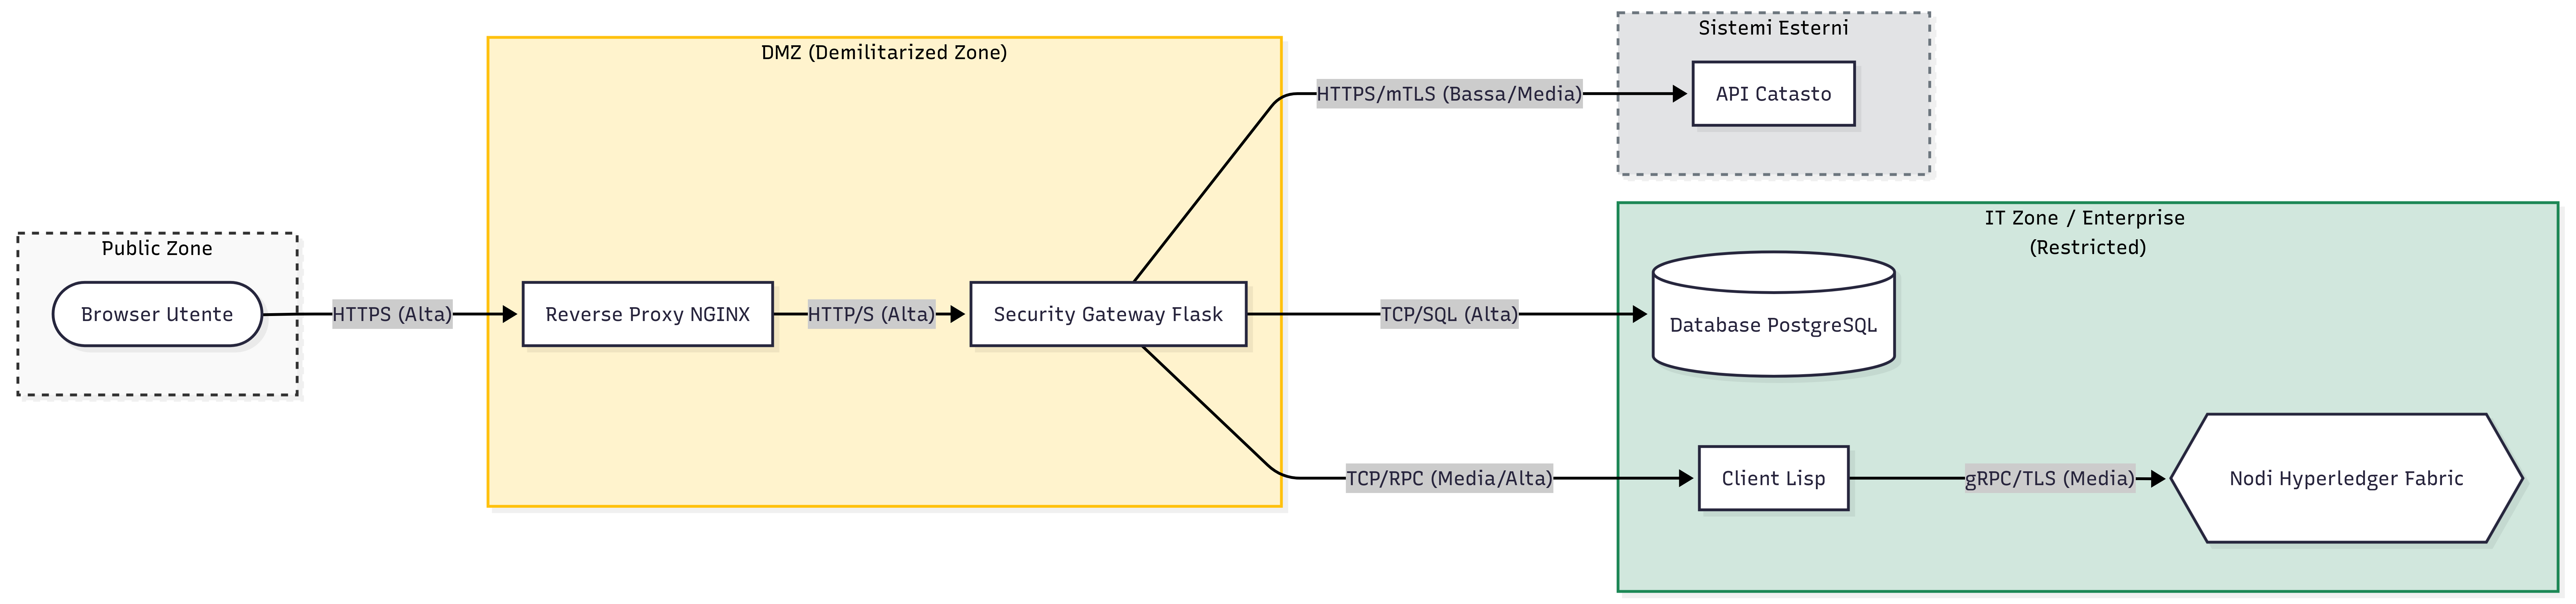
\includegraphics[width=1\textwidth]{img/threatmodelbuysellchaingraph.png}
    \caption{Grafo dell'infrastruttura}
    \label{fig:graph}
\end{figure}

\newpage

\begin{table}[ht!]
\centering
\footnotesize
\setlength{\tabcolsep}{3pt}
\renewcommand{\arraystretch}{1.15}
\begin{tabularx}{\textwidth}{X X X X X}
\toprule
\textbf{Sorgente} & \textbf{Destinazione} & \textbf{Protocollo} & \textbf{Frequenza} & \textbf{Motivazione / Logica di Business} \\
\midrule
Browser Utente & Reverse Proxy (DMZ) & HTTPS & Alta & Navigazione piattaforma, consultazione grid aste, login e invio offerte. Traffico cifrato TLS 1.3. \\
Reverse Proxy & Security Gateway & HTTP/S & Alta & Inoltro delle richieste decifrate (o ri-cifrate internamente) verso il server Flask per l'elaborazione. \\
Security Gateway & Database (IT Zone) & TCP/SQL & Alta & Validazione credenziali, recupero RBAC, lettura/scrittura dati anagrafici off-chain tramite SQLAlchemy. \\
Security Gateway & Client Lisp (IT Zone) & TCP/RPC & Media/Alta & Traduzione delle chiamate REST in primitive (\texttt{AddKV}, \texttt{GetKV}) per l'interazione con la Blockchain. \\
Client Lisp & Nodi Fabric (IT Zone) & gRPC/TLS & Media & Invocazione dello Smart Contract, proposta di transazioni e interrogazione dello stato del Ledger. \\
Security Gateway & API Catasto (Esterno) & HTTPS/mTLS & Bassa/Media & Chiamata sincrona per la certificazione e la validazione dei dati di un immobile in fase di creazione asta. \\
\bottomrule
\end{tabularx}
\caption{Mappatura dettagliata dei flussi di comunicazione autorizzati (Conduits) tra gli asset.}
\end{table}

\newpage

\section{Dall'Architettura alla Baseline Comportamentale (Operating Envelope)}
L'obiettivo di questa fase è usare la topologia di BuySellChain per definire cosa costituisce un comportamento di rete \textit{normale}.  
La normalità non è un punto singolo, ma un inviluppo operativo continuo (\textit{operating envelope}).  
La classificazione degli eventi deve quindi distinguere tra \textbf{Normal}, \textbf{Deviazione Lieve}, \textbf{Deviazione Forte} e \textbf{Unknown}.

\subsection{Definizione della Baseline Qualitativa}
Le comunicazioni attese vengono modellate come relazioni lecite tra asset, con frequenza temporale e intensità prevista.

\begin{table}[h]
\centering
\small
\renewcommand{\arraystretch}{1.4}
\begin{tabularx}{\textwidth}{>{\hsize=0.30\hsize\bfseries}X >{\hsize=0.17\hsize}X >{\hsize=0.13\hsize}X >{\hsize=0.40\hsize}X}
\toprule
Relazione Normale & Quando & Intensità & Note \\
\midrule
Frontend Web \(\rightarrow\) Security Gateway & Sempre (Sì) & Alta & Navigazione utenti, login, invio offerte. \\
Security Gateway \(\rightarrow\) DB Off-Chain & Sempre (Sì) & Alta & Validazione utenze, recupero RBAC, lettura dati GDPR. \\
Security Gateway \(\rightarrow\) Rete Fabric (via Client Lisp) & Sempre (Sì) & Media & Invocazione Smart Contract per registrazione aste/offerte. \\
Security Gateway \(\rightarrow\) API Catasto & Giorno/Notte (Sì) & Bassa/Media & Verifica validità immobili, chiamate asincrone/sincrone. \\
Utente Esterno \(\rightarrow\) DB Off-Chain & Mai (No) & Nulla & Deviazione topologica grave (violazione segmentazione). \\
Security Gateway \(\rightarrow\) Backup Storage & Notte (Sì) & Alta & Sincronizzazione pianificata dei dati Off-Chain. \\
\bottomrule
\end{tabularx}
\caption{Baseline qualitativa dei flussi leciti (Operating Envelope).}
\end{table}

\newpage

\subsection{Finestra di Telemetria Osservata (Dataset di Esempio)}
Si considera una finestra temporale campione con log estratti da firewall e Security Gateway.

\begin{table}[h]
\centering
\footnotesize
\renewcommand{\arraystretch}{1.35}
\begin{tabularx}{\textwidth}{>{\hsize=0.10\hsize\bfseries}X >{\hsize=0.28\hsize}X >{\hsize=0.24\hsize}X >{\hsize=0.12\hsize}X >{\hsize=0.10\hsize}X >{\hsize=0.16\hsize}X}
\toprule
Time & Source & Dest & Proto & Pkts & Status \\
\midrule
10:15 & Frontend Web (IP vari) & Security Gateway & HTTPS & 340 & ok \\
10:16 & Security Gateway & DB Off-Chain & TCP & 510 & ok \\
10:17 & Security Gateway & API Catasto & HTTPS & 15 & ok \\
10:18 & IP Pubblico (sconosciuto) & DB Off-Chain & TCP & 45 & fail \\
10:20 & Frontend Web (singolo IP) & Security Gateway & HTTPS & 850 & retry \\
03:05 & Security Gateway & Backup Storage & TCP & 1500 & ok \\
03:10 & Security Gateway & IP Pubblico (sconosciuto) & HTTPS & 2200 & ok \\
\bottomrule
\end{tabularx}
\caption{Finestra di telemetria osservata per la classificazione delle deviazioni.}
\end{table}

\subsection{Valutazione Deviazioni e Classificazione}
Gli eventi non pienamente compatibili con la baseline vengono classificati con severità e motivazione.

\begin{table}[h]
\centering
\footnotesize
\renewcommand{\arraystretch}{1.4}
\begin{tabularx}{\textwidth}{>{\hsize=0.30\hsize\bfseries}X >{\hsize=0.10\hsize}X >{\hsize=0.10\hsize}X >{\hsize=0.15\hsize}X >{\hsize=0.35\hsize}X}
\toprule
Evento & Compatibile & Score & Classificazione & Dato utile (giustificazione) \\
\midrule
10:18 IP Pubblico \(\rightarrow\) DB & No & Forte & Attacco & Log firewall: violazione grave della segmentazione. Il DB non deve ricevere traffico diretto dall'esterno. \\
10:20 Frontend \(\rightarrow\) Gateway & No & Medio & Fault / Attacco & Log autenticazione API: anomalia volumetrica da singolo IP. Possibile credential stuffing oppure errore client. \\
03:05 Gateway \(\rightarrow\) Backup & Parziale & Lieve & Unknown & Log schedulazione: trasferimento massivo atteso di notte, ma senza audit completo resta non conclusivo. \\
03:10 Gateway \(\rightarrow\) IP Sconosciuto & No & Forte & Attacco & Ispezione connessioni: invio dati verso destinazione esterna non censita. Forte indicatore di data exfiltration. \\
\bottomrule
\end{tabularx}
\caption{Classificazione delle deviazioni rispetto alla baseline comportamentale.}
\end{table}

\newpage

\subsection{Debrief Finale di Sicurezza}
\paragraph{Asset più critico e deviazione più grave.}
L'asset più critico resta lo \textbf{Smart Contract} su Fabric, poiché governa transazioni irreversibili di valore e proprietà.  
Le deviazioni più gravi osservate sono:
\begin{itemize}
    \item \texttt{03:10 Gateway \(\rightarrow\) IP Sconosciuto}
    \item \texttt{10:18 IP Pubblico \(\rightarrow\) DB}
\end{itemize}
Entrambe indicano potenziale data breach e fallimento dei controlli perimetrali di base.

\paragraph{Deviazione più ambigua.}
\texttt{10:20 Frontend \(\rightarrow\) Gateway} è ambigua: può essere un \textit{fault} applicativo (retry anomali) oppure un brute-force mirato. Senza log applicativi dettagliati, la decisione non è deterministica.

\paragraph{Quando la risposta corretta è ``Unknown''.}
Nel caso \texttt{03:05 Gateway \(\rightarrow\) Backup}, il volume elevato notturno è coerente con job leciti di backup ma, in assenza di evidenze di audit, la classificazione prudente resta \textbf{Unknown} per ridurre falsi positivi.

\paragraph{Controllo by-design prioritario.}
La \textbf{Network Segmentation} rigorosa (DMZ + reti virtuali isolate) riduce i falsi negativi e limita il blast radius. In questo modello, eventi come \texttt{IP Pubblico \(\rightarrow\) DB} devono essere bloccati nativamente dal perimetro (\textit{default deny}).

\begin{quote}
\itshape
``Detection non significa indovinare attacchi. Significa ridurre l'incertezza fino a una decisione difendibile.''
\end{quote} 




\end{document}